\documentclass[tikz,border=8pt]{standalone}
% Shared look for every TikZ diagram. Load with \input{../../tools/tikz-style.tex}
\usepackage[T1]{fontenc}
\usepackage{lmodern}
\renewcommand{\sfdefault}{lmr}  % diagrams use the same serif as the text
\usetikzlibrary{arrows.meta, positioning, shapes.geometric, calc, fit, backgrounds}
\definecolor{cblue}{HTML}{4C78A8}
\definecolor{corange}{HTML}{F58518}
\definecolor{cgreen}{HTML}{54A24B}
\definecolor{cred}{HTML}{E45756}
\definecolor{cpurple}{HTML}{B279A2}
\definecolor{cgrey}{HTML}{6B6B6B}
\tikzset{
  every picture/.style={font=\sffamily, line width=1.2pt},
  box/.style={draw=#1, fill=#1!12, rounded corners=4pt, align=center, inner sep=7pt, minimum height=1.1cm},
  box/.default=cgrey,
  arrow/.style={-{Stealth[length=3mm]}, draw=cgrey, line width=1.4pt},
  title/.style={font=\sffamily\bfseries\Large},
  note/.style={font=\sffamily\small, text=cgrey, align=center},
}
\AtBeginDocument{\hyphenpenalty=10000 \exhyphenpenalty=10000}

\begin{document}
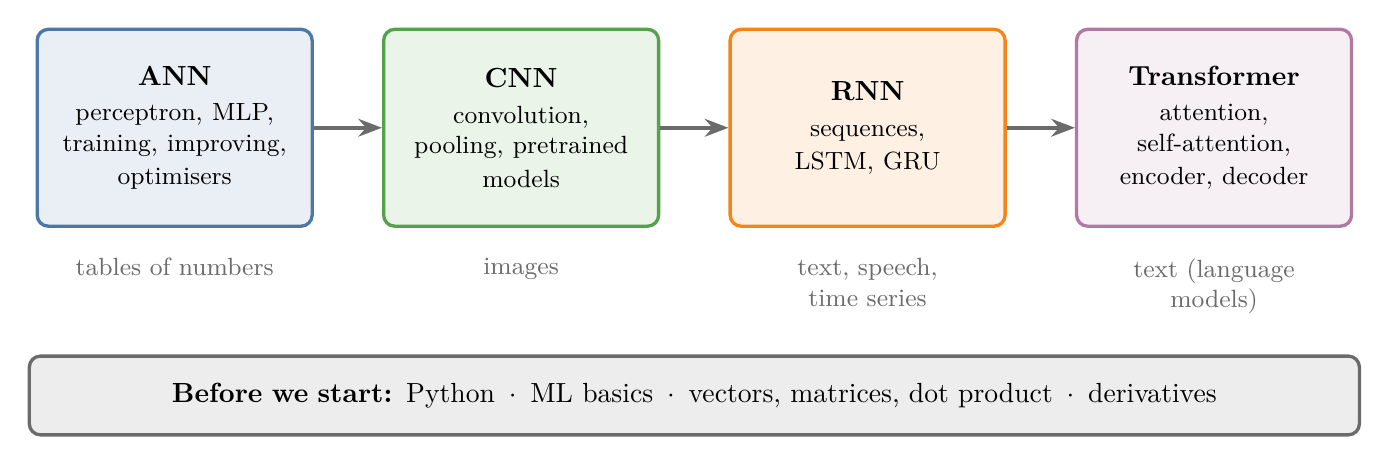
\begin{tikzpicture}[part/.style={box=#1, minimum width=3.3cm, minimum height=2.5cm, text width=3.0cm}]
  \node[part=cblue]   (ann) at (0,0)    {\textbf{ANN}\\[2pt]{\small perceptron, MLP,\\training, improving,\\optimisers}};
  \node[part=cgreen]  (cnn) at (4.4,0)  {\textbf{CNN}\\[2pt]{\small convolution,\\pooling, pretrained\\models}};
  \node[part=corange] (rnn) at (8.8,0)  {\textbf{RNN}\\[2pt]{\small sequences,\\LSTM, GRU}};
  \node[part=cpurple] (trf) at (13.2,0) {\textbf{Transformer}\\[2pt]{\small attention,\\self-attention,\\encoder, decoder}};
  \draw[arrow] (ann) -- (cnn); \draw[arrow] (cnn) -- (rnn); \draw[arrow] (rnn) -- (trf);
  \node[note, below=0.25cm of ann] {tables of numbers};
  \node[note, below=0.25cm of cnn] {images};
  \node[note, below=0.25cm of rnn] {text, speech,\\time series};
  \node[note, below=0.25cm of trf] {text (language\\models)};
  \node[box=cgrey, text width=16.4cm, minimum height=1.0cm] (pre) at (6.6,-3.4)
    {\textbf{Before we start:}\enspace Python\enspace$\cdot$\enspace ML basics\enspace$\cdot$\enspace vectors, matrices, dot product\enspace$\cdot$\enspace derivatives};
\end{tikzpicture}
\end{document}
